\section{Targets}
\label{sec:ui_targets}

\begin{figure}[H]
    \hspace*{-2.5cm}
    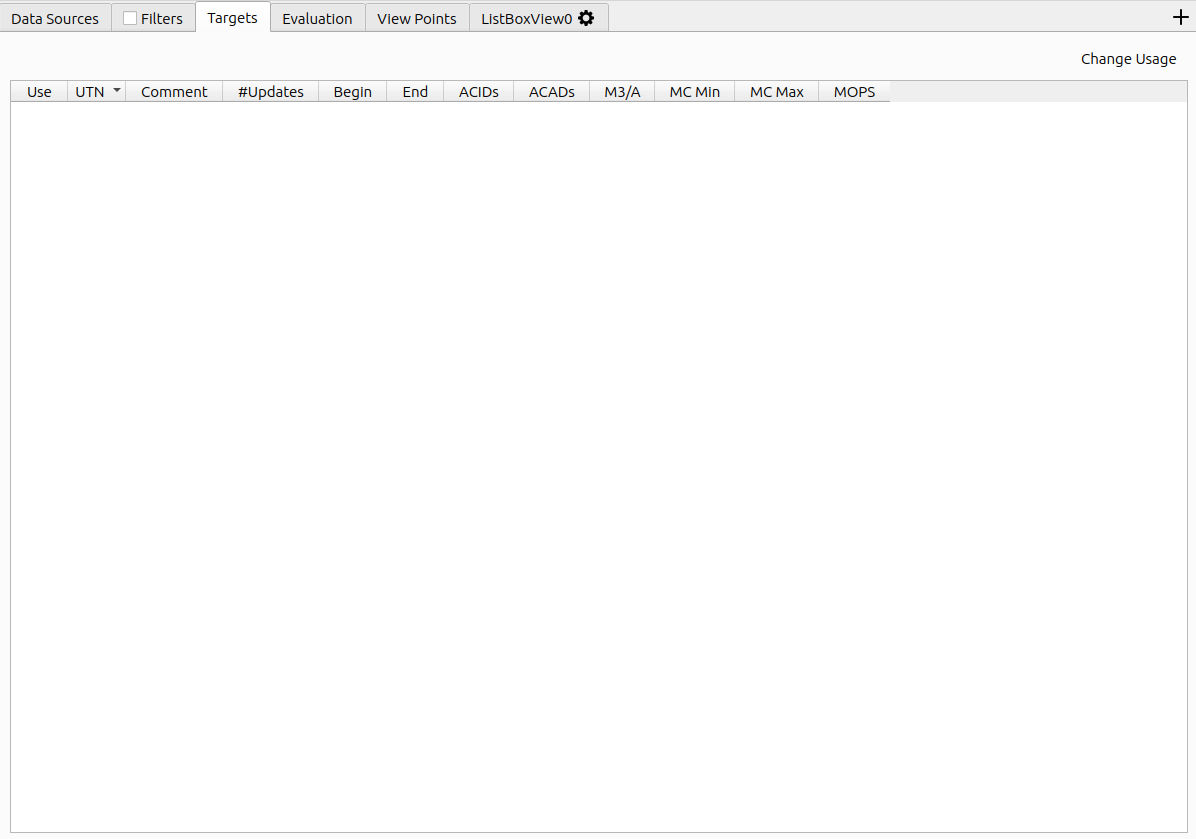
\includegraphics[width=19cm,frame]{figures/ui_targets.png}
  \caption{Targets Overview}
\end{figure}

In this tab, all existing targets are shown. If no associations were calculated, the list is empty. \\

The following columns exist:

\begin{itemize}  
\item Use: Checkbox defining if the target should be used in the evaluation
\item UTN: Unique Target Number
\item Begin: First timestamp of UTN
\item End: Last timestamp of UTN
\item \#All: Sum number of target reports
\item \#Ref: Number of target reports in reference data
\item \#Tst: Number of target reports in test data
\item Callsign: Target identification(s)
\item TA: Target address (hexadecimal)
\item M3/A: Mode 3/A code(s) (octal)
\item MC Min: Mode C code minimum [ft]
\item MC Max: Mode C code maximum [ft]
\end{itemize}
\ \\

After running the calculate associations task, the table can look as follows:

\begin{figure}[H]
  \hspace*{-2cm}
    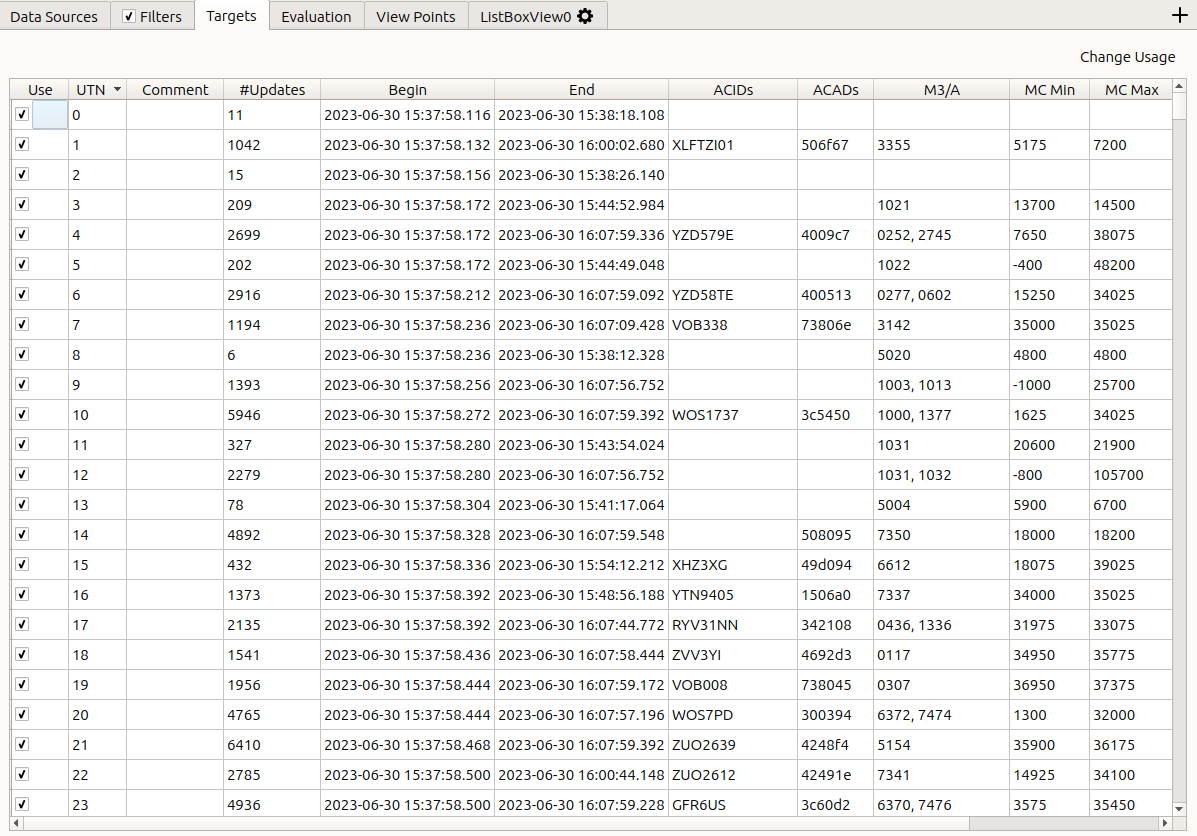
\includegraphics[width=18cm,frame]{figures/ui_targets2.png}
  \caption{Targets tab with calculated associations}
\end{figure}

When clicking a target, all data associated to the respective target is loaded.
